%%%%%%%%%%%%%%%%%  Debut du fichier Latex  %%%%%%%%%%%%%%%%%%%%%%%%%%%%%%
\documentclass[a4paper,12pt,onecolumn]{article}

%%% Pour un texte en francais

%%\usepackage[applemac]{inputenc}
%\usepackage[francais]{babel}
	         % encodage des lettres accentuees
\usepackage[T1]{fontenc}
\usepackage[utf8]{inputenc}          % encodage des lettres accentuees
%\usepackage{graphicx}
%%\usepackage{graphicx} \def\BIB{}
\usepackage[paper=a4paper,textwidth=140mm,left=2.7cm,right=2.7cm,top=2.8cm,bottom=2.8cm]{geometry}
\usepackage{multicol}
\usepackage{graphicx,wrapfig,lipsum} 
%\def\BIB{}
\usepackage[font=footnotesize]{caption}
\usepackage{subcaption}
\usepackage[pdftex]{hyperref}
\usepackage{natbib}
\usepackage{url}
\usepackage{changepage}
\usepackage{xspace}
\usepackage{perpage} %the perpage package
\MakePerPage{footnote} %the perpage package command
\hypersetup{
    colorlinks,%
    citecolor=black,%
    filecolor=black,%
    linkcolor=black,%
    urlcolor=blue     % can put red here to visualize the links
}


\DeclareUnicodeCharacter{00A0}{ }

%%% Quelques raccourcis pour la mise en page
\newcommand{\remarque}[1]{{\small \it #1}}
\newcommand{\rubrique}{\bigskip \noindent $\bullet$ }

\newcommand{\ignore}[1]{}

\renewcommand*\rmdefault{iwona}

\pagenumbering{gobble}

\newcommand{\sgx}{SgXB\xspace}
\newcommand{\sfxt}{\textsc{sfxt}}
\newcommand{\sg}{Sg\xspace}
\newcommand{\co}{CO\xspace}
\newcommand*{\hmxb}{HMXB\@\xspace}
\newcommand*{\rlof}{RLOF\@\xspace}
\newcommand*{\ns}{NS\@\xspace}
\newcommand*{\bh}{BH\@\xspace}
\newcommand*{\eg}{e.g.\@\xspace}
\newcommand*{\ie}{i.e.\@\xspace}
\newcommand*{\aka}{a.k.a. \@\xspace}

%\bibliographystyle{abbrvnat}
%\setcitestyle{authoryear,open={((},close={))}}

%\renewcommand{\thefootnote}{\roman{footnote}}

% -------------------------------------------------
\newcommand{\horrule}[1]{\rule{\linewidth}{#1}} % Create horizontal rule command with 1 argument of height

\title{	
\vspace*{-2cm}
\normalfont \normalsize 
El Mellah Ileyk \\ [25pt] % Your university, school and/or department name(s)
\horrule{0.5pt} \\[0.4cm] % Thin top horizontal rule
\huge Research\\ % The assignment title
\horrule{2pt} \\[0.5cm] % Thick bottom horizontal rule
}
%\author{El Mellah Ileyk} % Your name
\date{\tiny }%\normalsize\today} % Today's date or a custom date
% -------------------------------------------------

%\makeatletter
%\def\@xfootnote[#1]{%
%  \protected@xdef\@thefnmark{#1}%
%  \@footnotemark\@footnotetext}
%\makeatother

\begin{document}

%\bibpunct{[}{]}{;}{n}{,}{,}

%%%%%%%%%%%%%%%%%%%%%%%%%  PREMIERE PAGE %%%%%%%%%%%%%%%%%%%%%%%%%%%%%%
%%% DANS CETTE PAGE, ON REMPLACE LES INDICATIONS ENTRE CROCHETS [...]
%%% PAR LES INFORMATIONS DEMANDEES
%%%%%%%%%%%%%%%%%%%%%%%%%%%%%%%%%%%%%%%%%%%%%%%%%%%%%%%%%%%%%%%%%%%%%%%

\maketitle
\thispagestyle{empty}

\vspace*{-1cm}

Because most stars belong to a multiple stellar system, stellar evolution in binary systems is a topic of prime importance to shed light both on the planets which orbit them and on the galaxies which host them. Stars do not only impact their surroundings when they perform thermonuclear fusion but also as stellar remnants, once the core has long shut down, especially when they are orbited by a close-by stellar companion. In this case, the interplay between the two bodies gives birth to spectacular phenomena which help us to understand the specificities of each body. 

One of the most impressive possible outcomes of the evolution of binary systems are X-ray binaries. They host a compact object - a neutron star (\ns) or a black hole (\bh) - orbiting a stellar companion whose gas is accreted by the former and emits copious amounts of X-rays. Since the discovery of the first extrasolar X-ray source in the early sixties \citep{Giacconi1962}, continuous observations of these systems have revealed a broad range of spectral and photometric behaviors with a special emphasis on their incredible time variability : flares, hysteresis loops in hardness-luminosity diagrams, off-states, quasi-periodic oscillations... The core of my research activity has been to explore the possible origins of this time variability. 

The observation of these systems is made possible thanks to satellites funded, designed and maintained by international collaborations. By the end of the next decade, the ESA Athena X-ray observatory will provide unprecedented insights on high energy phenomena taking place in X-ray binaries (scientific goals 8.3 and 8.4 and observatory scientific goals 3) but also in Active Galactic Nuclei. Meanwhile, the harvest of data being still obtained by predecessors like Chandra or XMM-Newton constantly enlarges the number of X-ray binaries identified. The diversity of behaviors observed requires a versatile though constraining set of models. Given the level of complexity of the Physics at stake in X-ray binaries, we need to supply the analytical approach with a complementary tool : high resolution numerical simulations of fluid dynamics, enabled by the surge in modern computational capacities. Supercomputers have been widely established in the research landscape for the last 15 years and now offer a brand new approach. 

As a daily user and advocate of this new scientific method, I have learned how to tune numerical analogues of astrophysical objects, in close partnership with European observers. These models require specific efforts to accurately reproduce the phenomena we wish to investigate, and yield results which must be interpreted and checked with particular care. I describe in the present statement the conclusions derived during my research activity and how a position of Astronome-adjoint would enable me to extend my studies further.

%During my PhD, I characterized the structure of uniform wind accretion onto compact objects in binary systems. In my first year of postdoc, I extended this work by accounting for realistic micro-structure of the wind from the stellar companion.
\subsection*{Selected skills}

On top of my academic education in Physics, my experience in research made me develop extended skills including but not limited to :

\begin{adjustwidth}{-0.5cm}{-0.5cm}
\begin{itemize} %[labelindent=1.3em, labelsep=-3cm,leftmargin=*]
\setlength\itemsep{-0.2em}
\setlength{\itemindent}{-1em}
\item[] \underline{Astrophysics }
\begin{itemize}
\setlength\itemsep{-0.2em}
\setlength{\itemindent}{-2em}
\item radiative hydrodynamics (HD) : line-driven winds, optically thin and thick cooling/heating
\item magneto-HD (MHD) : magnetosphere of a degenerate star
\end{itemize}
\item[] \underline{Computational Fluid Dynamics} 
\begin{itemize}
\setlength\itemsep{-0.2em}
\setlength{\itemindent}{-2em}
\item hyperbolic partial differential equations : Riemnann solvers, slope limiters 
\item High Performance Computing (HPC) : parallelization, multithreading, Tier-1 clusters 
\end{itemize}
\item[] \underline{Data analysis } 
\begin{itemize}
\setlength\itemsep{-0.2em}
\setlength{\itemindent}{-2em}
\item Python programming : NumPy, SciPy, pandas
\item 3D data visualization softwares : VisIt, Paraview, Tecplot
\item Graphical User Interface (GUI) : applets (with Wolfram language and Spyre framework)
\item Fourier and wavelet data analysis
\end{itemize}
\item[] \underline{Code development}
\begin{itemize}
\setlength\itemsep{-0.2em}
\setlength{\itemindent}{-2em}
\item advanced Fortran 2003 programming : procedure pointers
\item Perl and bash scripting : pre-processors, serial job runs
\item parallel code debugging : Allinea Forge's DDT
\item parallel code profiling and optimization : VampirTrace 
\item interactive and responsive web design : HTML5, CSS and Javascript
\end{itemize}
\item[] \underline{Project management } 
\begin{itemize}
\setlength\itemsep{-0.2em}
\setlength{\itemindent}{-2em}
\item version control : GIT
\item team time scheduling : Gantt charts
\end{itemize}
\end{itemize}
\end{adjustwidth}

\subsection*{Research activity report}

\subsubsection*{PhD research activity}

\indent During my PhD, I focused on mass transfer in binaries via wind accretion, the low angular momentum counterpart of the more comprehensively understood Roche lobe overflow (RLOF) mechanism. Supergiant X-ray binaries (\sgx), where a compact object (generally a \ns) orbits an evolved O/B supergiant, are the ideal stage for wind accretion to occur. Indeed, the latter displays intense outflows, a fraction of which being captured by the \ns. The rapid increase since the late 2000’s in the number of \sgx \citep{Walter15} and the ambiguous status of the newly discovered Supergiant Fast X-ray Transients \citep[SFXT,][]{Negueruela2006} only increased the appeal of this burning topic.\\ \\
\indent In a first attempt to better understand the wind accretion process, I confronted the analytical prescriptions derived by Bondi, Hoyle and Lyttleton \citep[BHL,][]{Hoyle:1939fl,Bondi1944} to a more realistic HD representation of the flow. To do so, I used and developed the explicitely flux-conserving finite volume transport code \texttt{MPI-AMRVAC} \citep{Xia2017}. The new version I contributed to now addresses HD or magneto-HD (MHD) problems, in Cartesian, cylindrical or spherical geometry, with or without polytropic prescriptions, source terms, etc. For wind speeds similar to the ones observed in \sgx ($\sim$1,000km$\cdot$s$^{-1}$), the main challenge is the contrast between the scale at which the gravitational beaming of the fast inflow by the accretor becomes significant (the accretion radius) and the size of the compact accretor, typically 4 to 5 orders of magnitude smaller. Since most of the emitted light comes from the immediate vicinity of the accretor, it is important to follow the flow through these scales. To uniformly resolve the incoming planar flow, I implemented a radially stretched grid in a 2D spherical geometry. With suitable boundary conditions, I reached a numerically relaxed state and spanned the 5 required orders of magnitude thanks to the computing time I was granted on the CINES Tier-1 cluster (see Figure\,\ref{fig:zoom_BHL}). In \cite{ElMellah2015}, we characterized the structure of the flow, which forms a stable detached bow shocked as it is beamed towards the wake of the accretor, and the dependence of the mass accretion rate on the Mach number of the inflow. For the first time, we monitored the flow deep enough to confirm the analytical prediction by \cite{Foglizzo1997} concerning the topology of the inner sonic surface (where the shocked flow becomes supersonic again) which has to be anchored into the accretor.\\ \\
\begin{figure}[!b]
\begin{center}
\hspace*{-0.8cm}
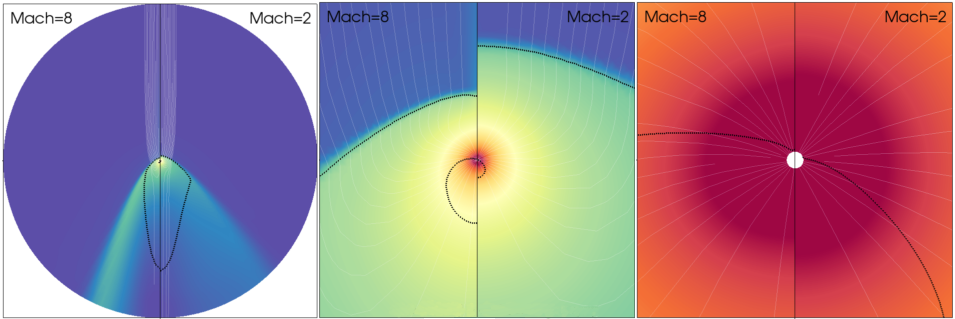
\includegraphics[height=6cm, width=17cm]{Figures/zoom_BHL.png}	
\caption{Successive zoom in on the innermost parts of a planar flow (coming from the top) being deflected by a central accretor for different Mach numbers at infinity. In white are represented the streamlines while the dotted black lines represent the Mach-1 surfaces. The colormap is logarithmic mass density.}
\label{fig:zoom_BHL}
\end{center}
\end{figure}
\indent In a realistic \sgx though, the incoming wind is not planar due to the orbital bending. It carries a non-zero angular momentum which could, in some cases, lead to the formation of a wind-capture disc. To identify the favorable configurations, I designed a model of supersonic line-driven wind propagation in \sgx, coupling the stellar, orbital, wind and accretion parameters \citep{ElMellah2016a}. I identified the minimal set of dimensionless degrees of freedom of the problem to optimally explore the space of parameters. This investigation showed how sheared and beamed the wind is when it enters the region around the accretor where the shock is expected to develop - i.e. where the ballistic assumption breaks up and where HD simulations similar to the ones above are required. The need to connect the orbital scale motion, essentially ballistic, and the accretion region, centered on the compact object, became apparent.\\



\subsubsection*{Postdoctoral research activity}

\begin{figure}[!b]
\begin{subfigure}{0.45\columnwidth}
  \centering
%  \hspace*{-1cm}
  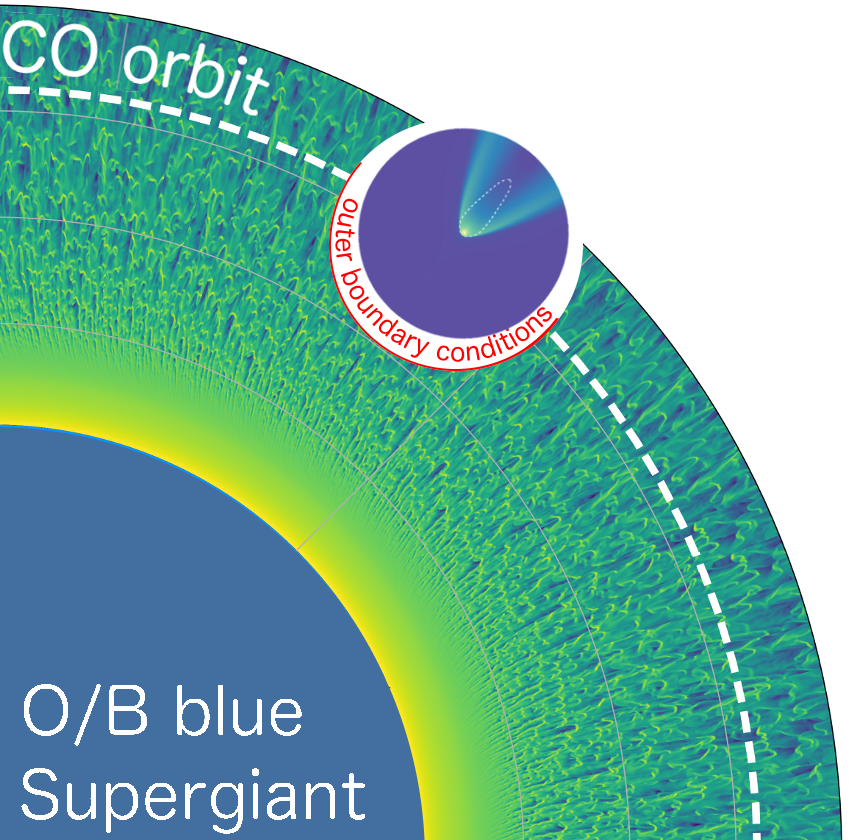
\includegraphics[height=7cm]{Figures/config_SgXB_clumps.png}	
\end{subfigure}%
\begin{subfigure}{0.45\columnwidth}
  \centering
  \hspace*{0.25cm}
  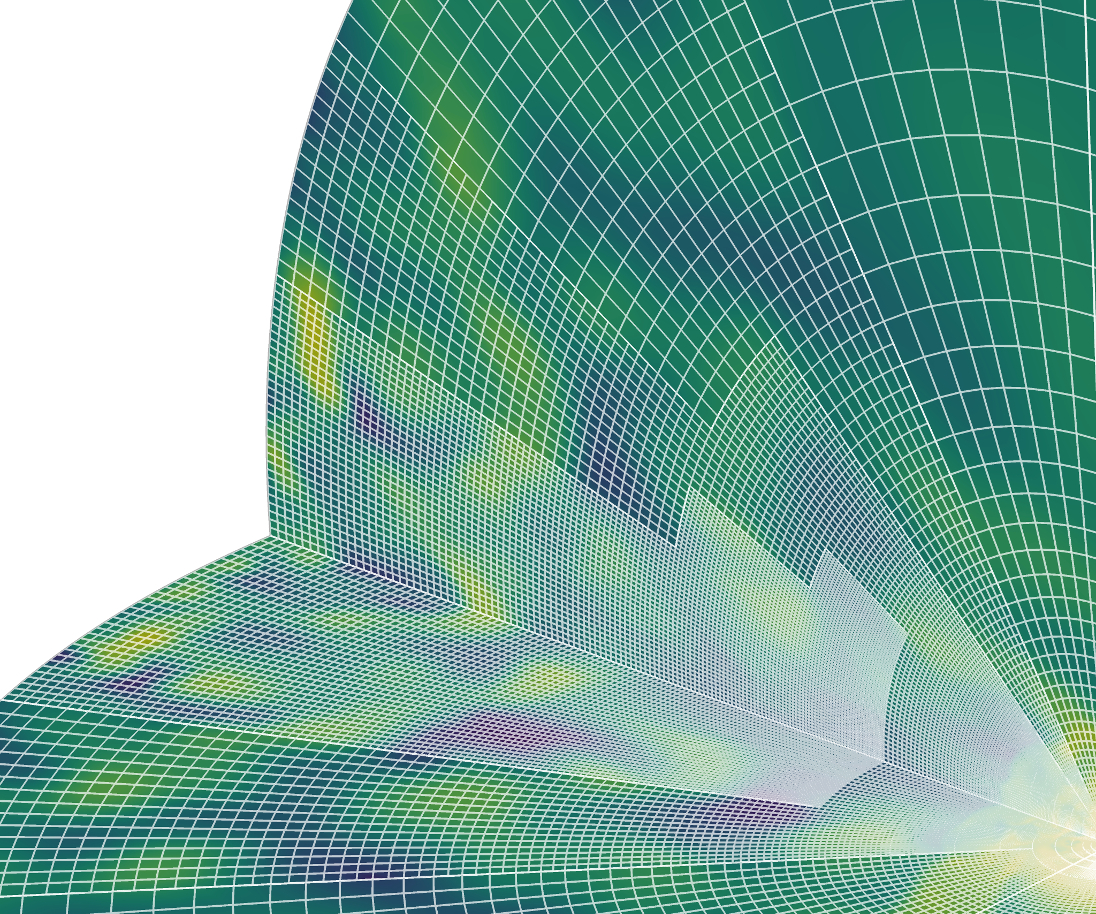
\includegraphics[height=7cm]{Figures/mesh.jpeg}	
\end{subfigure}
\caption{(\textit{left}) Principle of the clumpy wind accretion simulations : we inject into the simulation space (upper right insert) a wind whose micro-structure has been computed out of radiative HD simulations by \cite{Sundqvist2017}. (\textit{right}) Two-slices representation of the upstream hemisphere of the simulation space, with the wind coming from the upper left. We overlaid a logarithmic density map to show the typical size of the inhomogeneities to resolve. The accretor lies in the bottom right corner.}
\label{fig:config_SgXB_and_mesh}
\end{figure}

\indent Since the beginning of my postdoctoral activity one year ago, I started to consider more realistic internal structure for the incoming wind in \sgx than the uniform flow I had worked with during my PhD. Indeed, the line-driven winds of massive stars are notoriously inhomogeneous, due to the line-deshadowing instability \citep{Owocki1984a} which leads to the formation of internal shocks. The serendipituous accretion of these overdense regions, or clumps, has been suggested as a possible explanation to the time variability of the X-ray luminosity in \sgx, of the order of 100 peak-to-peak. Using a 2D pseudo-planar grid sampling a restricted angular region, \cite{Sundqvist2017} recently managed to compute the dimensions and shapes of the clumps, for an isolated massive stars. To evaluate the impact of clumps on the accretion process, I plunged a compact object in the wind ("CO" in the left panel in Figure\,\ref{fig:config_SgXB_and_mesh}), at different orbital separations, and injected the corresponding wind computed by \cite{Sundqvist2017} within the simulation space (right panel in Figure\,\ref{fig:config_SgXB_and_mesh}). By coupling the stretching of the mesh to the Adaptive Mesh Refinement (AMR) of \texttt{MPI-AMRVAC}, I could design 3D spherical setups spanning several orders of magnitude at an affordable computational cost and resolve small scale off-centered features like clumps injected from the upstream hemisphere. In \cite{ElMellah}, we followed the clumps as they cross the shock and monitored the time variability at the inner border of the simulation space, corresponding approximately to the dimensions of the \ns magnetosphere. With this work, we discovered how tempering the shock could be, which led to variations of the inner mass accretion rate an order of magnitude smaller than the observed variations of the X-ray luminosity in these systems. Thus, if the stochastic variations at low X-ray luminosity seem to match the variability induced by the clumps alone (see Figure\,\ref{fig:diag}), the high luminosity levels can only be reached due to other underlying mechanisms, possibly within the \ns magnetosphere \citep[\eg the propeller effect,][]{Bozzo2016}. Concerning the column density levels, we retrieve average values compatible with what has been observed recently in Vela X-1 by \cite{Grinberg2017}.
\begin{wrapfigure}[27]{l}{0.5\textwidth}
\vspace*{-0.2cm}
\captionsetup[subfigure]{labelformat=empty}
\centering
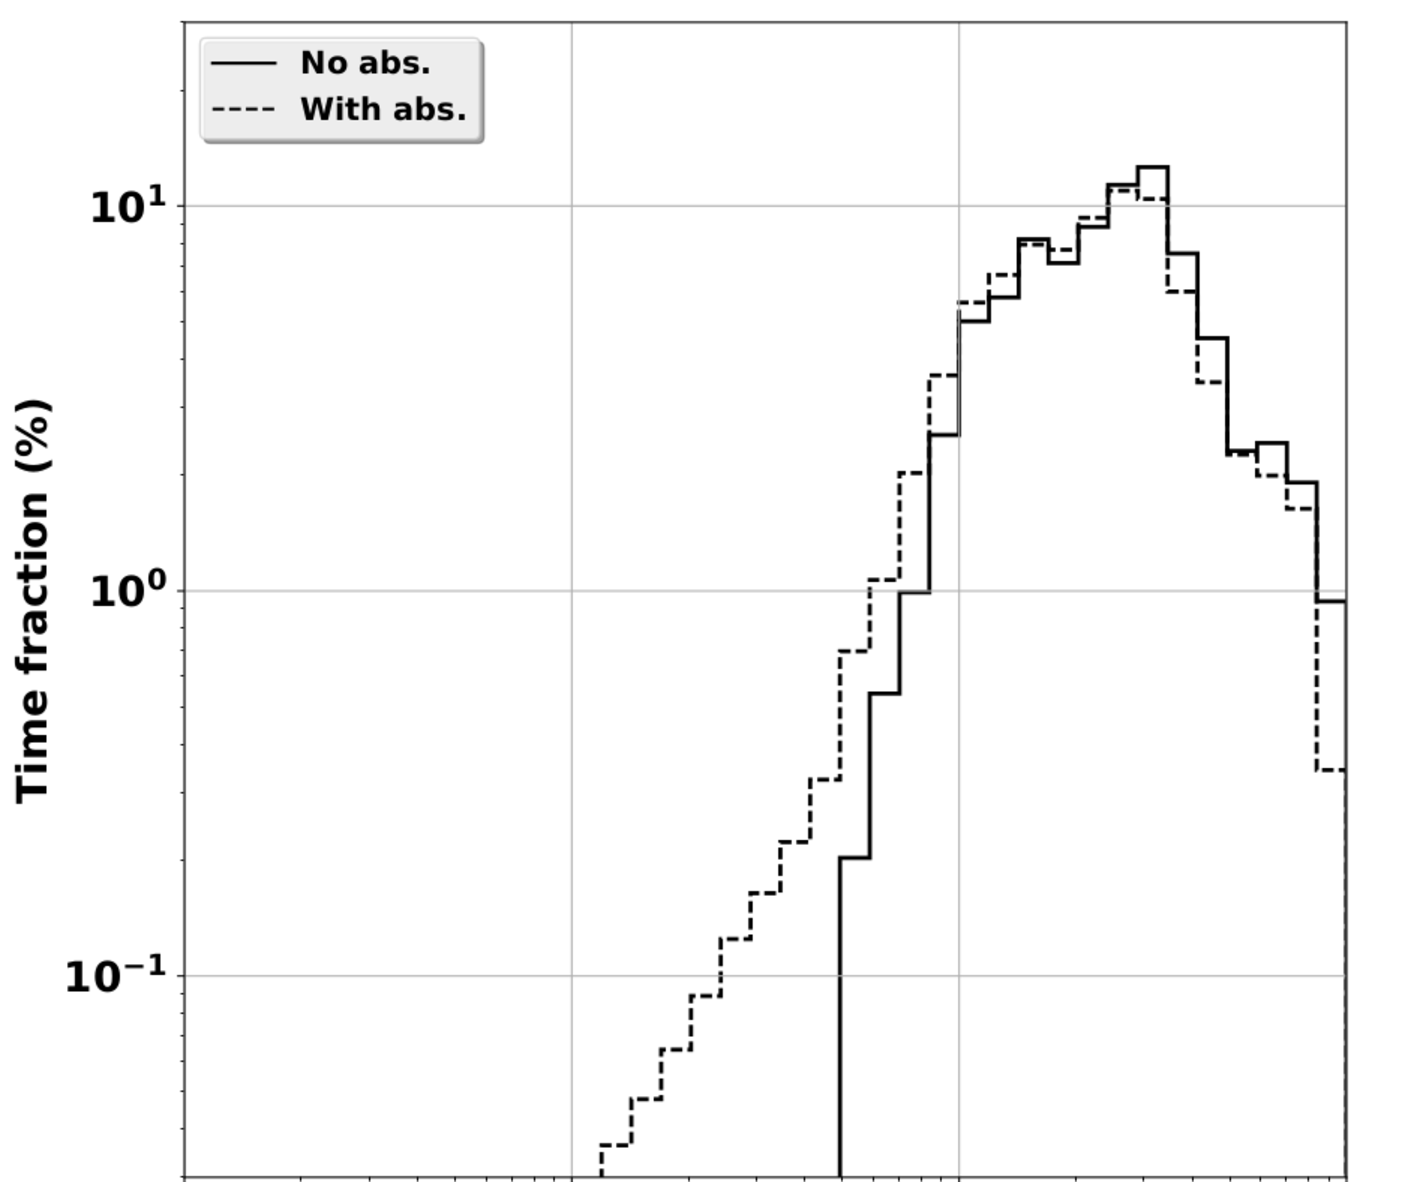
\includegraphics[width=0.45\textwidth]{Figures/lum_diag.pdf}
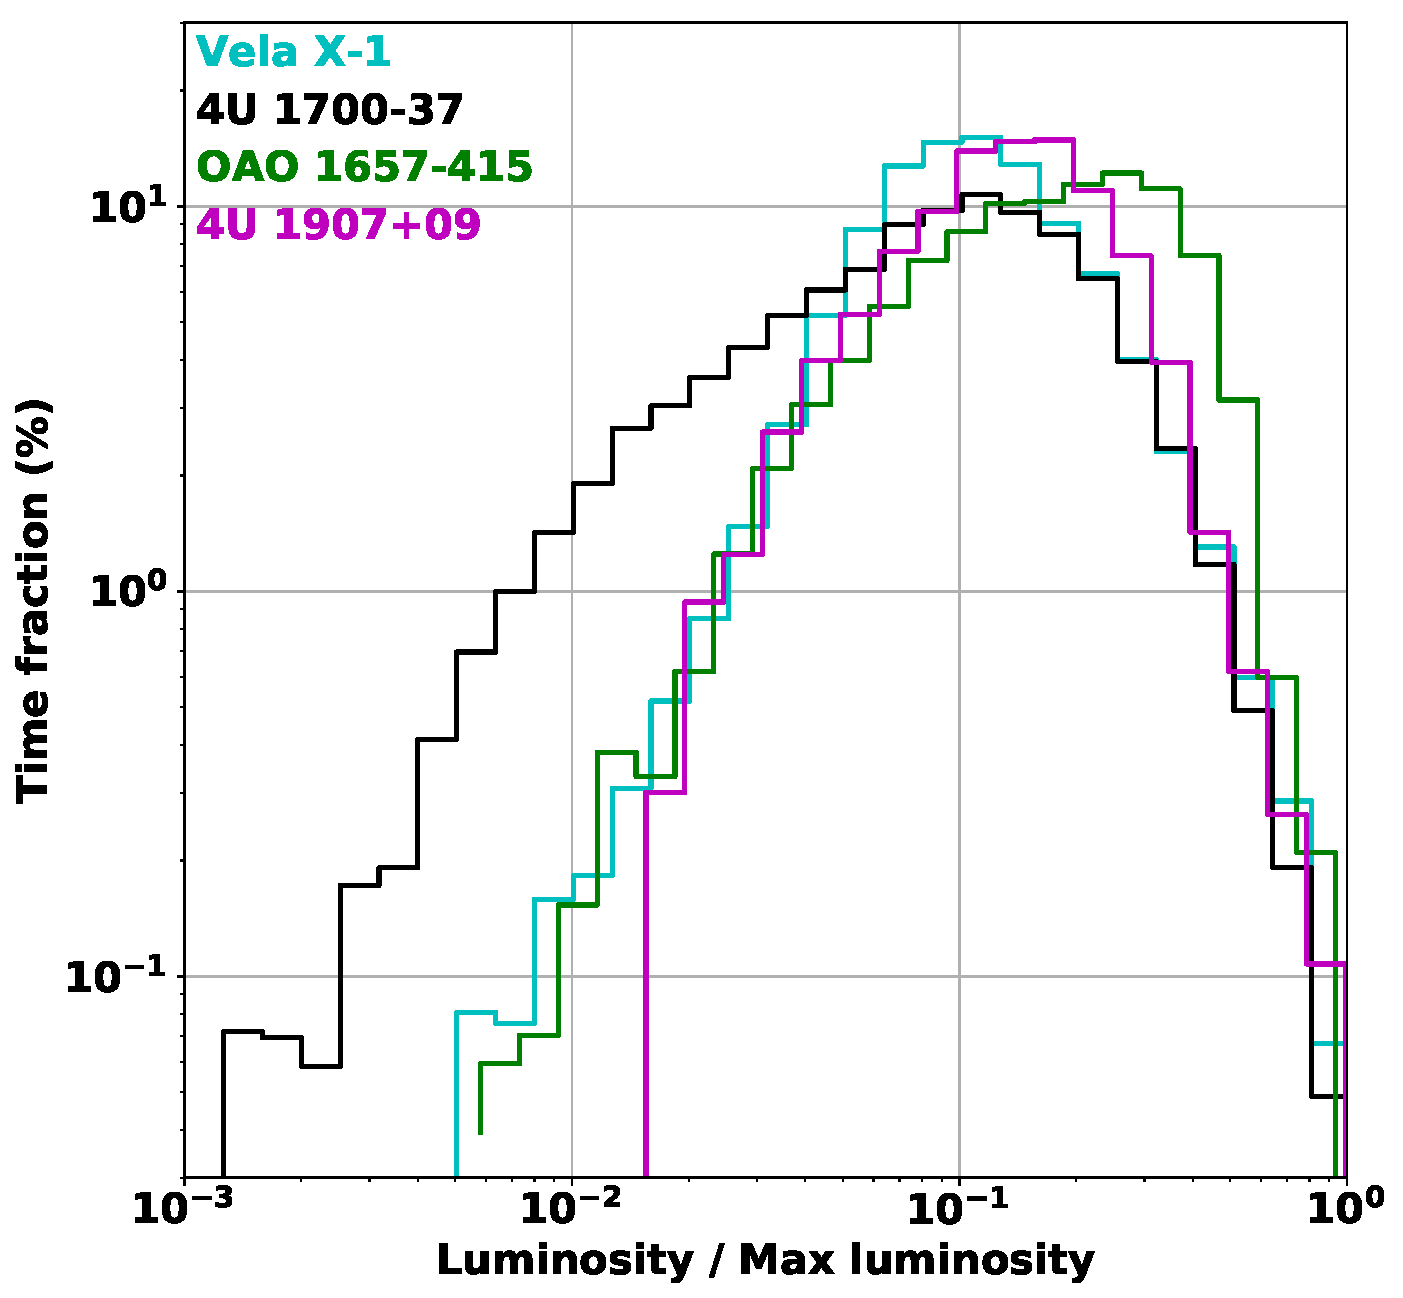
\includegraphics[width=0.45\textwidth]{Figures/obs_diag.pdf}
\caption{(upper panel) Simulated luminosity histograms, with and without accounting for absorption. (bottom panel) Observed luminosity histograms for 4 classic \sgx \citep[from][]{ElMellah}.} \label{fig:diag}
\end{wrapfigure} 
%\begin{wrapfigure}{r}{7.2cm}
%\vspace*{-1.5cm}
%\hspace*{0.1cm}
%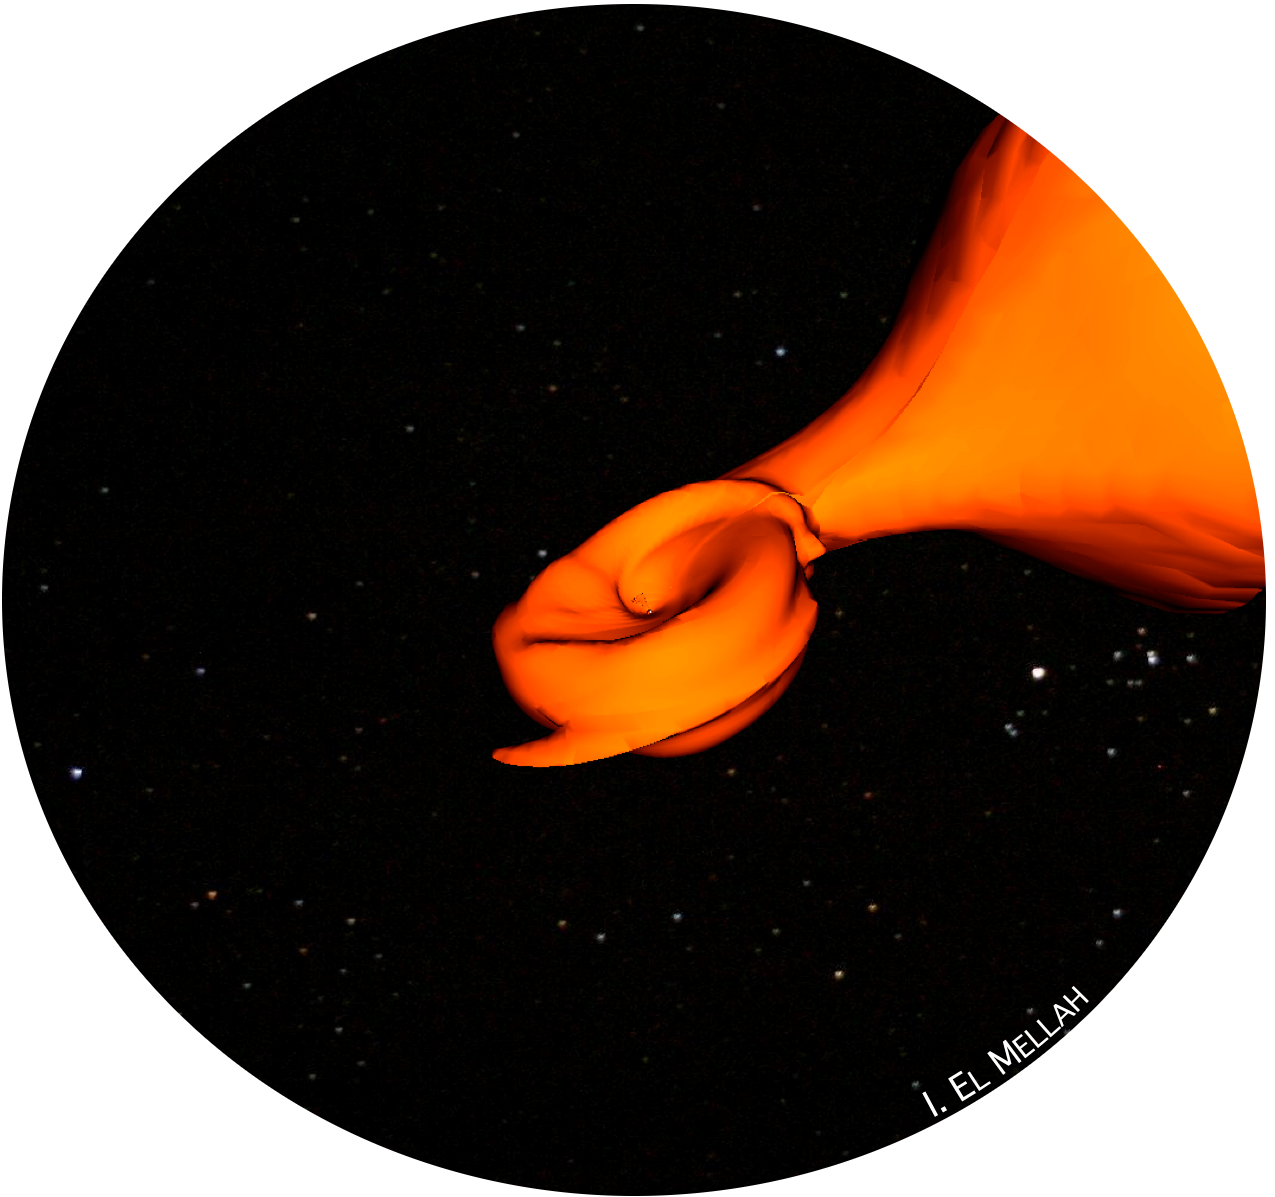
\includegraphics[height=7.1cm]{Figures/RLOF.png}
%\caption{Isodensity surface of a 3D flow from a \rlof star (upper right) to an accretor, 1,000 times smaller than the orbital separation between the two bodies.}
%\label{fig:bow2.5d}
%\end{wrapfigure} 
\phantom{m}\\
\indent I also participated to \cite{Grinberg2017} to evaluate the time variability associated to unaccreted clumps passing by the line-of-sight and concluded that this type of micro-structure within the wind can not explain by itself the variations in column density we observed. This contribution has been made possible thanks to the \href{http://www.issibern.ch/teams/stellarwindxray/}{ISSI team} I have been invited to join in February 2017, at the occasion of their second workshop in Bern. In November 2017, I gathered at ESAC (Madrid) with Peter Kretschmar (ESAC), Silvia Mart\'{i}nez-N\'{u}\~{n}ez (IFCA), Victoria Grinberg (ESTEC) and Felix F\"{u}rst (ESAC) to provide the theoretical expertise to the X-Wind collaboration which aims at developing further the work carried out by the ISSI team : providing a more comprehensive view of the stellar wind in Supergiant X-ray binaries thanks to a synergy between specialists in winds of isolated massive stars and specialists in high mass X-ray binaries.\\ \\
\phantom{m}\\ \\
\indent Eventually, in \cite{Xia2017}, I carried out a numerical validation of the stretched grid implementation I had made during my PhD by confronting quantitative simulation results of Bondi spherical accretion to the analytical expectations on the mass accretion rate and the location of the sonic point for different adiabatic indexes. We also studied the propagation of a trans-Alv\'enic wind from the solar surface to the Earth orbit to validate the compatibility of the stretched grid with the MHD solver and Powell's method for the cleaning of the divergence of the magnetic field.\\

\subsection*{Research project}

Since most of the X-ray emission we observe comes from the immediate vicinity of the accretor, we want to study the high energy phenomena at stake within a few hundreds of Schwarzschild radii around the accretor. In SgXB, the magnetic field of the accreting NS can no longer be discarded in this zone. We now need to investigate other sources of time variability than the clumps to interpret the observations :
\begin{itemize}
\item the presence of a transient disc-like structure around the accretor could lead to specific disc instabilities (\eg the magneto-rotational instability).
\item magnetic and centrifugal gatings at the edge of the NS magnetosphere are expected to contribute to break up the accreted flow, along with thermodynamical considerations which modulate the entry within the NS magnetosphere.
\item the X-ray ionizing feedback from the immediate vicinity of the accretor alters the dynamics of the wind at the orbital scale.
\end{itemize}
These 3 trails form the backbone of my research project in the following years. If it is mostly aimed at \sgx and SFXT, it has also ramifications to similar systems such as Cataclysmic Variables (CV), low mass X-ray binaries or Be X-ray binaries. Thanks to the suited numerical framework I contributed to develop over the last years, we can aspire to obtain, by the end of the next decade, a consistent overview of the mass transfer process, from the Dantean stellar surface down to the magnetic vicinity of a NS, if not the relativistic surroundings of a black hole. Current missions (\eg XMM-Newton, Chandra and Integral) provide us with the guiding constrains of our numerical investigations, while future ones (\eg SVOM, LOFT and Athena) will bring unprecedented observations which will confront theoretical expectations even further.

%\newgeometry{left=2.1cm,right=2.1cm,top=2.8cm,bottom=2.8cm}
%\newpage

\subsubsection*{Wind-capture discs}

\begin{wrapfigure}{r}{7.2cm}
\vspace*{-1.5cm}
\hspace*{0.1cm}
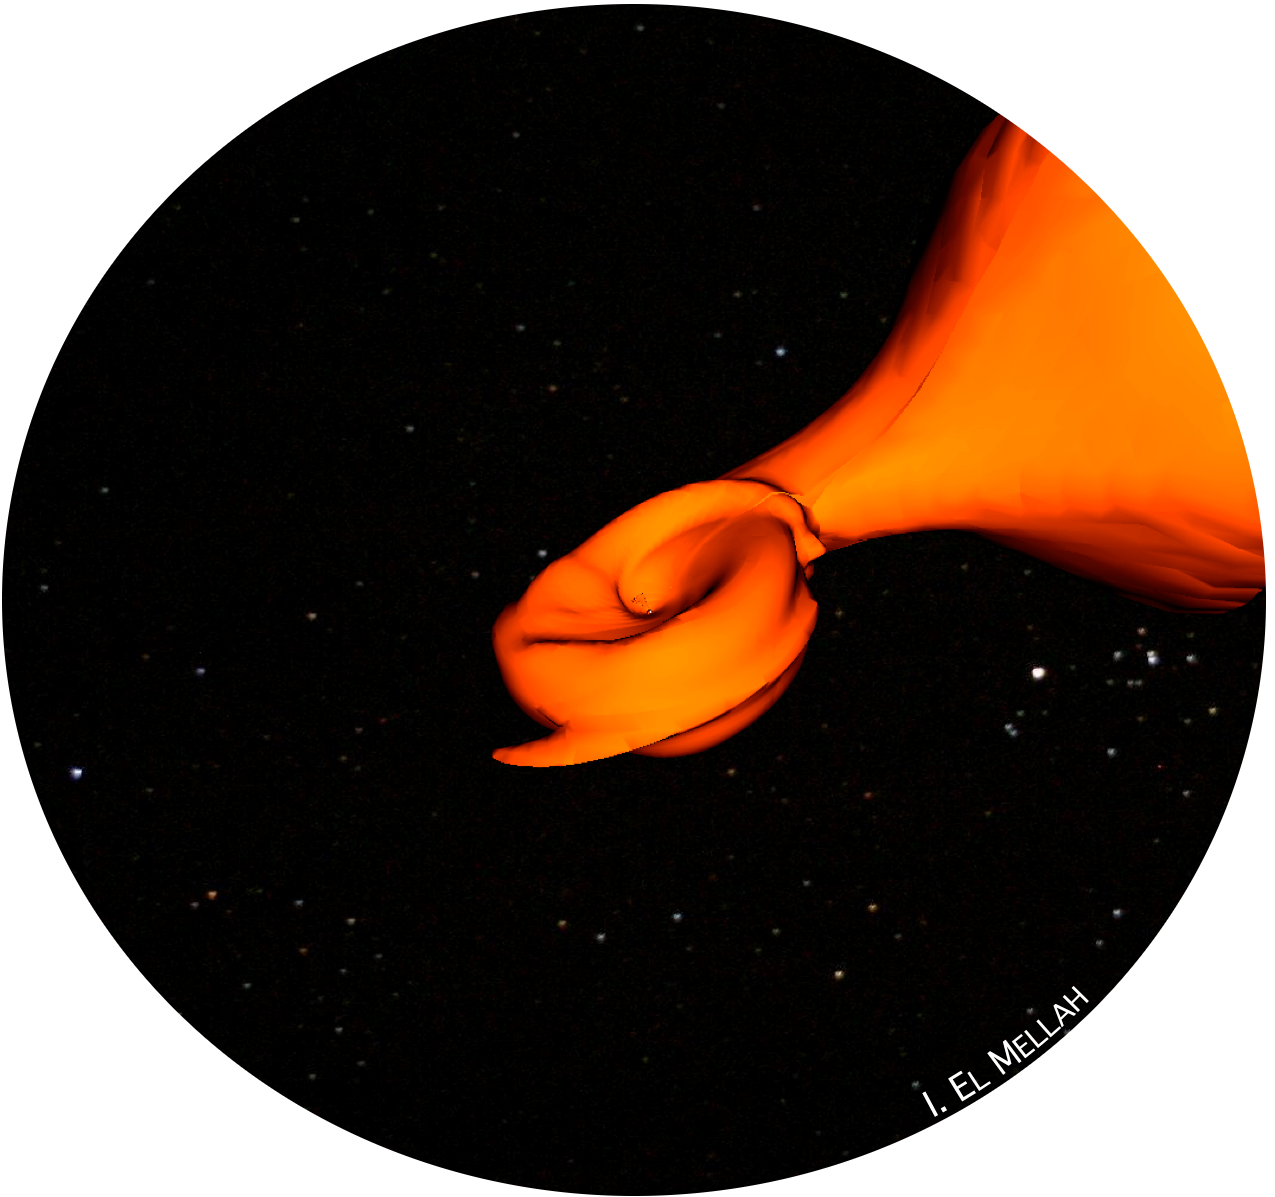
\includegraphics[height=7.1cm]{Figures/RLOF.png}
\caption{Isodensity surface of a 3D flow from a \rlof star (upper right) to an accretor, 1,000 times smaller than the orbital separation between the two bodies.}
\label{fig:bow2.5d}
\end{wrapfigure} 

The first step of this research project addresses the capacity of the accreted flow to form a disc, depending on the speed of the flow compared to the orbital speed. In the low speed-limit, a \rlof star pours matter at the first Lagrangian point directly into the Roche lobe of the accretor (see Figure\,\ref{fig:bow2.5d}). The flow winds up around the accretor and forms a large permanent disc. In the high-speed limit, long thought to be valid for \sgx, the line-driven wind coming from a high mass donor star carries little angular momentum : the flow structure is described by the BHL solution and no disc is expected. However, \cite{Mohamed2011} laid the foundations for a treatment of the intermediate case or \textit{wind-RLOF}. In \cite{ElMellah2016a}, I adapted it for \sgx. Recent observational and numerical results on the wind speed in the classic \sgx Vela X-1 suggest that neither of the 2 aforementioned asymptotic cases apply \citep{Gimenez-Garcia2016,Sander2017} and a wind-RLOF approach is required. I plan to study this case to identify the conditions of formation of wind-captured discs (see Figure\,\ref{fig:wind-RLOF}). Discs are known to be fruitful landscapes for a plethora of instabilities which might partly contribute to the time variability in some \sgx.\\ \\

\begin{wrapfigure}{l}{7.2cm}
\vspace*{-0.5cm}
\hspace*{0.1cm}
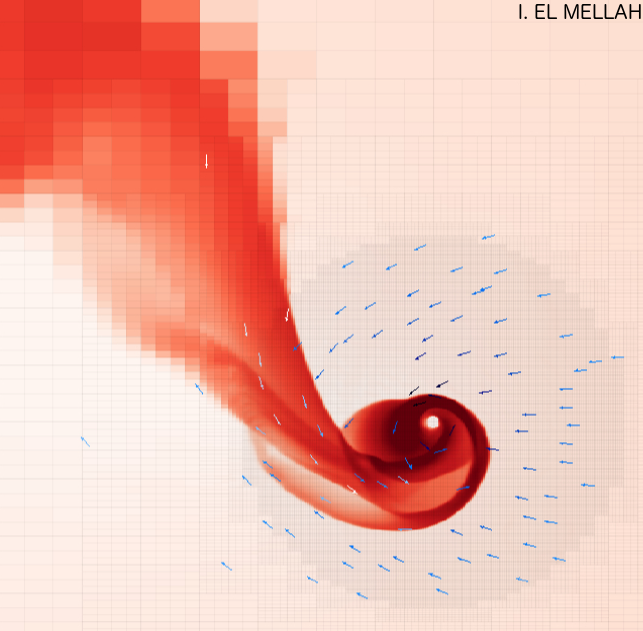
\includegraphics[height=7.1cm]{Figures/wind-RLOF.png}
\caption{Density and velocity map of a slow wind (coming from the right) being accreted onto a compact object. The detached bow shock becomes a disc-like structure.}
\label{fig:wind-RLOF}
\end{wrapfigure} 

%\indent This problem would make the most of ray-tracing tools such as \texttt{GYOTO} \citep{Vincent2011} whose main developers work at the LUTh (Eric Gourgoulhon) or at the neighboring LESIA (Fr\'ed\'eric Vincent, Thibaut Pomard \& Guy Perrin). Indeed, for a \sgx hosting a black hole such as Cygnus X-1, progresses on the structure of the disc and its environment would bring, once processed with \texttt{GYOTO}, new insights on the photometric and spectroscopic properties. Also, low angular momentum accretion onto a compact object is a subject of prime importance for Sagittarius A* which is observed with the GRAVITY instrument managed, among others, by the LESIA.

\indent These questions strongly connect to the domains of interest of the Observatoire de Paris, in particular of the LUTh and the LESIA. Indeed, accretion of low angular momentum flow onto a compact object might accurately describe the accretion process taking place in the Galactic Center, Sagittarius A*, observed with the GRAVITY instrument managed, among others, by the LESIA. Furthermore, these simulations need to be processed with ray-tracing tools such as \texttt{GYOTO} \citep[developed among others by Fr\'ed\'eric Vincent now at the LESIA,][]{Vincent2011} to yield synthetic observations (\eg for Cygnus X-1). The insights it would bring on the environment of accreting compact objects would be valuable for the theoretical models developed at the LUTh (\eg by Eric Gourgoulhon or Fabrice Mottez). 

%\clearpage

%\newgeometry{left=2cm,right=2cm,top=2.6cm,bottom=2.6cm}

%\newpage

%To guarantee that we work with physically consistent accretion discs, I am now performing numerical simulations of RLOF configurations where the expanded atmosphere of the donor star is channeled into the Roche lobe of the accretor through the first Lagrangian point. This model includes a proxy on viscosity, similar to the one introduced by \cite{Shakura1973}, and energy losses through radiative cooling. The former stands for the turbulent viscosity associated to the magnetic rotational instability \citep{Balbus1991}. Together with spiral shocks, they participate to the evacuation of angular momentum which makes the accretion possible. The ballistic solution is then superseded by the actual formation of a disc around the accretor. Since the plasma largely exceeds 10,000K during the accretion process, a significant fraction of the elements is ionized. We make use of the SPEX cooling tables for solar abundances to compute the cooling function \citep{VanMarle2011}, which yields cooling rates large enough to impact the thickness of the flow. However, the numerically convenient optically thin assumption we currently make breaks up in the disc and must be complemented with a flux-limited diffusion method I plan to implement in \texttt{MPI-AMRVAC}. These improvements could first lead to insights concerning the origin of negative superhumps in cataclysmic variables \citep[CV, ][]{Murray1998}. Replacing the inner accretor with a \bh or a lowly magnetized NS, the wrapping of the disc could also be studied and numerical results obtained in the context of Smooth Particle Hydrodynamics simulations could be confronted \citep{Foulkes2006}. If the disc turns out to be misaligned with the orbital plane, it could have a serious impact on jet-launching conditions since a misalignement with the \bh spin is likely to induce a precession of the jets \cite{Liska2017}.

\subsubsection*{The NS magnetosphere}

\begin{wrapfigure}[13]{r}{5.2cm}
\vspace*{-1cm}
\hspace*{0.1cm}
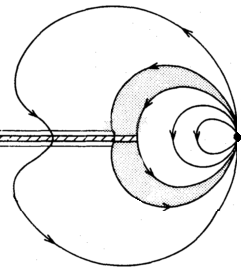
\includegraphics[height=5.1cm]{Figures/ghosh_lamb.png}
\caption{Truncation of the inner disc by the NS magnetosphere. From \cite{Ghosh1978}.}
\label{fig:ghosh}
\end{wrapfigure} 

The NS in \sgx are strongly magnetized since their young age did not allow for a significant decay of their pristine dipolar field. Within the magnetosphere, magnetically-funneled accretion onto the poles takes place. Yet, the contrast between the size of the NS and the orbital separation makes it challenging to develop a numerical setup suitable for magneto-hydrodynamical problems. To alleviate this obstacle, we started with Zakaria Meliani (LUTh) to study a family of binaries where the accretor is one hundred times larger and where the orbital separation is ten times smaller : cataclysmic variables, hosting a white dwarf (WD). These systems still retain the main qualitative ingredients as \sgx while being much more computationally affordable. In intermediate polars, a sub-class of CV, a RLOF star feeds an accretion disc truncated at its innermost border by the magnetic field of the accreting white dwarf (see Figure\,\ref{fig:ghosh}). The flow is then funneled to the WD poles where it is shocked and heated to high temperatures, emitting copious amounts of light. We are currently implementing a grey cooling method into our code, \texttt{MPI-AMRVAC}, to see the interplay between a physically-motivated stratified disc and the WD magnetic field. Coupled to the adaptive mesh stretched grid I developed during my PhD, this approach could improve our understanding of the WD spinning down. More generally, such a setup will be also used to set constrains on the disc reformation after a nova \citep{Ness2012} : with U Scorpii expected to go off in a couple of years, I started to collaborate with Jan-Uwe Ness (ESAC) to write together an observation proposal by summer 2018.\\
\indent This twofold setup also serves another purpose : diving into the magnetosphere of the accreting NS in \sgx, where the magnetic field is larger. Numerically, we recently implemented and validated a numerical algorithm of magnetic splitting generalized to non-potential fields \citep{Xia2017}. It enables us to handle more accurately the magnetic field evolution, in particular in magnetically-dominated plasmas, and to clean more easily the non-zero divergence. With this new feature available, we want to study how the innermost parts of the wind behave. Depending on how the magnetosphere radius compares with other characteristic length scales such as the accretion and corotation radii, the flow might be halted and cascade later on within the magnetosphere \citep{Bozzo2008}. We can now study this modulation with physical inputs accounting for the variability at the upper scales derived in \cite{ElMellah}. We also want to address the case where the NS magnetospheric radius is much larger, of the order of the accretion radius. How does it alter the shock? This topic connects to the studies on the NS structure which are conducted at the LUTh by J\'er\^ome Novak and collaborators.
 	
\subsubsection*{X-ray ionizing feedback}

In the European X-wind collaboration I joined early 2017, my role is to connect the information we get from state-of-the-art numerical simulations of line-driven winds of isolated massive stars to the variability of the X-ray emission and absorbing column density observed in \sgx. The next step to perform this connection in a self-consistent way is to evaluate the radiative influence of the X-rays emitted in the immediate vicinity of the accretor on the inflowing wind. Indeed, the efficiency of line-driven acceleration drops when the wind gets excessively ionized \ie as it gets closer from the accretor it feeds. In the continuation of \cite{Blondin1990}, \cite{Manousakis2015c} performed 2D simulations where they accounted for this effect but prescribed an a priori fixed X-ray luminosity. We aim at dynamically computing this X-ray luminosity from the mass accretion rate at the inner border of the large scale contrast simulation space introduced in \cite{ElMellah}. The X-wind collaboration workshop of October 2018 in Santander will be the occasion to confront these results to new observations, while our monthly telecons allow us to keep track of the intermediate steps performed by each of the 20 members or so.\\

Since the end of my PhD, I have built up multiple collaborations to embed the numerical tool into the scientific method, as a binder between the theoretical approach, limited by the mathematical tools available, and the observational approach, limited by the instruments at our disposal. Thanks to the HPC technologies, Computational Astrophysics has ushered in a particularly exciting period to address a wide range of questions pertaining to accretion, from Active Galactic Nuclei to X-ray binaries and planetary formation. Concomitantly, the multiple confirmed detections of gravitational waves from coalescing compact objects have urged even more the community to evaluate the impact of binarity on the evolutionary tracks of massive stars. To this extent, high mass X-ray binaries represent a decisive stage whose understanding would shed light on many fundamental questions, from the scarcity of intermediate mass black holes to the equation-of-state of matter at supernuclear densities in neutron stars. A position as an \textit{astronome-adjoint} at the Observatoire de Paris, in LESIA or LUTh whose members show a shared interest in compact objects and their surroundings, would enable me to carry on this research program and reinforce the connections I built up with the scientific community in France. I would also strengthen the numerical expertise of the Observatoire de Paris-Meudon.\\



\vspace*{-0.5cm}
\subsubsection*{References}
{\def\section*#1{}
%\newgeometry{left=2cm,right=2cm,top=2.5cm,bottom=2.5cm}
\setlength{\bibsep}{5pt}
\footnotesize
\bibliographystyle{agsm}
\bibliography{/Users/Ileyk/Documents/Bibtex/research_statement_no_url}
}

\end{document}
%%%%%%%%%%%%%%%%%  Fin du fichier Latex  %%%%%%%%%%%%%%%%%%%%%%%%%%%%%%

